\chapter{Řešení návrhu desky plošných spojů}

\section{Napájecí část}

\subsection{USB-C}

Součástka J1 je zásuvka s datovým rozhraním USB 2.0. Použitý mikrokontrolér STM32U575 podporuje režim Full-Speed s přenosovou rychlostí 12 Mbit/s \cite[tab.~5 a~7]{st_an4879}. Pro funkci zvukové karty je důležitý požadovaný datový tok zvuku, např. pro stereofonní PCM při vzorkovací frekvenci 48 kHz a rozlišení 16 bitů vychází
\begin{equation}
    R_{\mathrm{PCM}} = f_s N C
    = 48\,000 \cdot 16 \cdot 2
    = 1\,536\,000\,\mathrm{bit/s}
    = 1{,}536\,\mathrm{Mbit/s},
    \label{eq:usb_audio_datovy_tok}
\end{equation}
kde $f_s$ je vzorkovací frekvence, $N$ počet bitů
na vzorek jednoho kanálu a $C$ počet kanálů. Výpočet nezahrnuje režii USB přenosu. Pro uvedený příklad poskytuje USB Full-Speed dostatečnou přenosovou kapacitu.

R14 a R15, oba s hodnotou 5,1 kOhm, připojují samostatně piny CC1 a CC2 k zemi. Podle těchto rezistorů zdroj rozpozná připojené zařízení jako příjemce napájení. Dva piny CC, každý s vlastním rezistorem, umožňují rozpoznání zařízení při obou orientacích zasunutí konektoru. D+ a D- tvoří diferenciální datovou dvojici USB 2.0. Vývody A6 a B6 jsou propojeny jako D+, vývody A7 a B7 jako D-. Toto propojení zajišťuje datové připojení při obou orientacích zasunutí konektoru \cite{espressif_usb_c}. U2 chrání datové vodiče a U9 chrání vodiče CC1 a CC2 před elektrostatickými výboji, které mohou vznikat při manipulaci s konektorem. Ochranné součástky omezují napěťové špičky a odvádějí proud výboje do ochranných cest. Jejich malá parazitní kapacita omezuje zatížení chráněných signálových vedení \cite{datasheet_usblc6_2,datasheet_tpd2e2u06}. Použití vnějších ESD ochran u USB rozhraní doporučuje STMicroelectronics v aplikační poznámce AN4879. Pro účinnou ochranu mají být umístěny co nejblíže zásuvce a připojeny krátkou cestou k zemní ploše \cite{st_an4879}.


\subsection{Lineární nabíječ akumulátoru s řízením napájecí cesty }
- vybranů akumulátor obsahuje vlastní ochranný modul PCM, podle dokumentace PCM zajišťuje ochanu před přebitím, nadměrným vybitím a nadproudem. Baterie nemá vlastní NTC termistor pro sledování teploty, má tedy pouze 2 piny, PLus a mínus. Mezi pin TS a GND je tedy osazen rezistor R11 = 10kOhm, udržující přípustnou úroveň na vstupu TS a umožňující nabíjení bez sledování teploty akumulátoru. Pevný odpor neposkytuje informaci o  teplotě baterie. 

- R11 osadit, ale umístit ho tak, aby byl na desce baterie, aby se dotýkal. R11 je umístěn na stranu přivrácené k akumulátoru s ohledem na pozdější možnost pozdějšího ozazení SMD termistoru. V základní variantě je osazem pevný rezistor 10 kOhm. Jeho náhrada za NTC termistor vyžaduje kompatibilní pouzdro, vhodnou odporovoou charakteristiku a zajištění tepelné vazby na akumulátor. 

- Současně je ale navržena ochrana tvořená obvodu DW01A a FS8205A umožňující použití jiného akumulátoru bez vlastního PCM modulu. Ochana je zapojena do proudové cesty i při použití baterie s vlastním PCM; vznikají tak dvě navazující ochrany

- DW01A pro vyhodnocení ochranných stavů a spínání tranzistorů, sleduje napětí a podmínky nadproudu. Prostřednictvím snímacího vstupu vyhodnocuje nadproudové podmínky, pokud se dosáhne ochranného prahu, začne ovládat tranzistory aby se přerušila cesta nabíení nebo vybíjení.

- FS8205A obsahuje 2 MOSFETy zapojené proti sobě, lze s nimi blokovat oba směry proudu baterie

- Koncové nabíjecí napětí je přibližně 4,2 V. Jako dolní provozní mez vybíjení je v návrhu uvažováno napětí 3,0 V. Dodržení této meze musí zajistit řízení přehrávače; BQ24074 nezajišťuje odpojení vybíjení právě při této hodnotě. Parametr \(V_{\mathrm{LOWV}}\approx3{,}0\,\mathrm{V}\) označuje přechod z přednabíjení do hlavního nabíjení.

- Pro akumulátor s kapacitou 1600 mAh odpovídá standardnímu nabíjecímu režimu 0,2 C proud 320 mA a režimu 0,5 C proud 800 mA. V navrženém zapojení je rezistorem R5 = 3,16 kohm nastaven typický nabíjecí proud přibližně 282 mA, tedy 0,176 C.

- nabíječ BQ24074 lineární nabíjecí obvod pro jeden Li-Ion/Li-pol článek

- průběh nabíjení: případné přednabíjení malým proudem, poté fáze konstantního proudu CC a pak fáze konstantního napětí CV, napětí v CV zůstává na koncovém nabíjecím napětí cca 4,2V a proud postupně klesá, po dosažení ukonřovacího proudu se nabíjení terminuje

- současná power path umožňuje současně nabíjet baterii a zároveň napájet přehrávač. Odběr přehrávače jde přes pin OUT, nabíješ stále sleduje nabíjecí proud baterie odděleně od odběru zařízení. ukonření nabíjení baterie je tedy možné i při současném spuštění zařízení. Při nedostatku dostupného vstupního proudu obvod upřednopstňuje napájení systému a snižkuje nabíjecí proud.

- nastavení nabíjecího proudu pomocí rezistoru R5: jde o 0,176C (platí pro kapacitu baterie 1600 mAh)
\begin{equation}
    I_{\text{CHG}} = \frac{K_{\text{ISET}}}{R_5} = \frac{890 \text{A}\Omega}{3160 \Omega} \approx 282 \text{mA}.
    \label{eq:ichg}
\end{equation}

- dva režimy napájení pomocí pinů EN2 (stáhnutý ke GND, vždy tedy logická 0) a pin EN1 řízený MCU STM32 a současně připojen na R2 = 100 kOhm k VBUS. Pokud je VBUS přítomný, ale je neaktivní řízení z MCU, výchozí stav je USB500, pokud EN2 = 0 (default) a EN1 = 1. POkud EN1 je stařen do logické nuly, nastaví se stav USB100. Vstupní limit je společný pro napájení přehrávače i nabíjení baterie. Po připojení USB se automaticky měnič zapne

- pin OUT: při dostatečném vstupním napájení je OUT regulovaný na cca 4,4V, baterie se mezitím nabíjí na 4,2V. síť ;"sys\_power" neposkytuje stabilizovaných 3,3V, bez vstupního napětí je tato větev napájena z baterie přes vnitřní tranzistor. Napětí 3,3V vytváří až navazující měnič.

- Bezpečnostní časovače jsou nastaveny rezistorem R7 = 68 kOhm připojeným mezi TMR a GND. Pro typickou hodnotu koeficientu \(K_{\mathrm{TMR}}=48\,\mathrm{s/k\Omega}\) vychází časový limit přednabíjení
\[
t_{\mathrm{PRECHG}}
=K_{\mathrm{TMR}}R7
=48\cdot68
=3264\,\mathrm{s}
=54{,}4\,\mathrm{min}.
\]
Časový limit hlavního nabíjení činí
\[
t_{\mathrm{MAXCHG}}
=10K_{\mathrm{TMR}}R7
=32640\,\mathrm{s}
\approx9{,}07\,\mathrm{h}.
\]
Jedná se o typické bezpečnostní limity, nikoli o předpokládanou dobu nabití akumulátoru. Při omezení nabíjecího proudu příslušnými regulačními smyčkami se časování zpomaluje. Překročení časového limitu vede k vyhodnocení poruchy.


- konfigurace kondenzátorů kolem 
C4 na vstupu IN 
C2 na výstupu OUT, oba kapacitu 4,7uF. Kondenzátor C3 mezi BAT a GND má 10 uF.

- tepelné ztráty lineárního nabíjení jsou podle P = (Uin - Ubat)\* Icharge, při 5V pro Uin, 3,7V Ubat a Icharge 282 mA vychází P = 0,37 W. tepelná regulace může snížit nabíjecí proud, podle datasheetu 9.3.5.8 je již zabudovaná v BQ24074, obvod sám sleduje svou vnitřní teplotu a reguluje nabíjecí proud.
Hondota P = 0,37 W představuje pouze ztráty spojené s nabíjecím proudem,

- odvod tepla z BQ24074 zajištěn propojením zemní mědí (GND) a exponované tepelné plošky pouzdra, podle doporučení návrhu DPS.

- zapojení je připraveno pro sledování teplopty akumulátoruy pomocí NTC termistoru připojeného třetím vývodem J2 na vstup TS

- z datasheetu byl vzán tento průběh nabíjení baterie LiIon pro ilustraci
\begin{figure}[htbp]
    \centering
    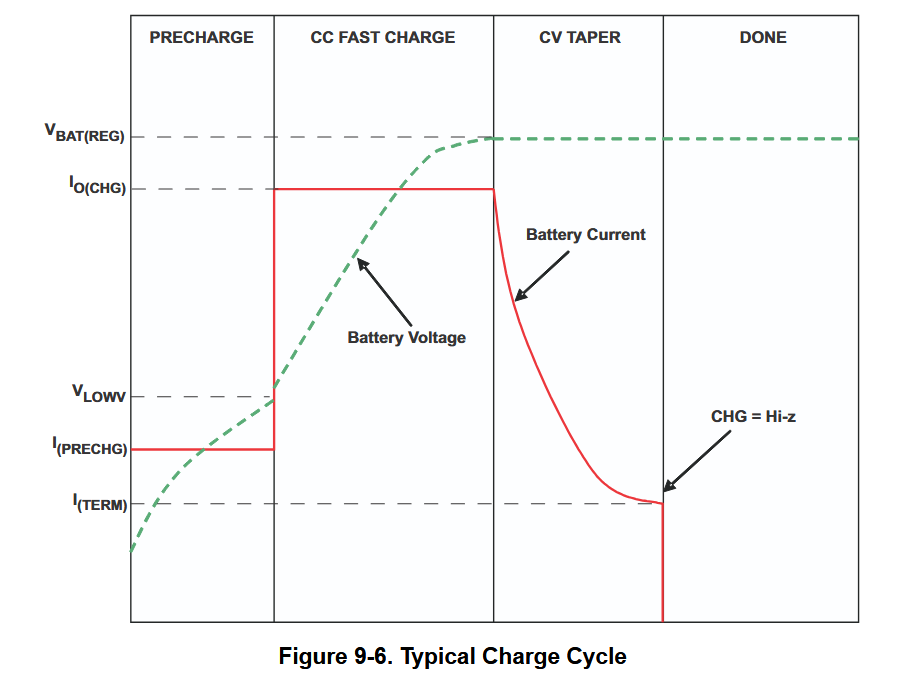
\includegraphics[width=0.8\textwidth]{obrazky/BQ24074_typical_charge_cycle.png}
    \caption{Typický nabíjecí cyklus Li-Ion baterie}
    \label{fig:BQ24074_typical_charge_cycle}
\end{figure}

Zelená přerušovaná křivka v grafu \ref{fig:BQ24074_typical_charge_cycle} představuje napětí na svorkách baterie UBat, červená křivka pak představuje proud jdoucí do baterie IBat. Osa X představující časovou osu, je schematická, nelze určit jednotlivou délku, skutečné hodnoty jednotlivých fází by mohly být doplněny měřením audio zařízení. Jde pouze o principiální ilustrativní průběh, ne o skutečnou měřenou charakteristiku. VBat(reg) zde představuje regulované koncové nabíjecí napětí, pro návrh přenosného audio přehrávače jde o 4,2 V. VLow je práh přechodu z přednabíjení do hlavního nabíjení, hodnota pro návrh  typicky 3,0V, s mezemi 2,9 V-3,1V. Io(chg) je nastavený proud nabíjecí fáze, nastavený podle schématu na 282 mA. IPrechg je proud přednabíjení, nastavený na 28 mA (0.1xIo) Iterm je proudový práh ukončení nabíjení, pro režim USB100 je to 9,3 mA, pro režim USB500 28,2mA. Pin ITERM je ponechán nezapojený, typický ukončovací proud činí proto přibližně 28,2 mA v režimu USB500 a 9,3 mA v režimu USB100.

\subsubsection{Precharge}
Jestliže má baterie před zahájením nabíjení napětí nižší než Vlowv, nabíječ nejprve použije malý proud IPrechg, proto je červená křivka průběhu nabíjení zde konstantní na jedné nízké úrovni. Náboj dodávaný nabíječem BQ24074 postupně zvyšuje napětí baterie (zelená postupně rostoucí křivka). Tento proces je zapotřebí, jestliže se baterie nachází v silně vybitém stavu, dodávání proudu IPrechg nemusí tedy být při každém nabíjení. Pokud je prah Vlowv překročen, poté nabíječ může zvýšit proud, začíná pak hlavní nabíjecí fáze. Vlow řídí pouze přechod z přednabíjecí řásti do plně nabíjecí (do fáze nabíjení konstantním proudem).

\subsubsection{Fast Charge CC}
CC = constant current, nabíječ udržuje nabíjecí proud přibližně na hodnotě Io(chg), napětí na baterii postupně roste. Proud nastavuje rezistor R5 ze schématu zapojení, podle rovnice \eqref{eq:ichg}. Jakmile je dosaženo napětí na betrii 4,2V, přejde se na další část nabíjení.

\subsubsection{CV Taper, nabíjení konstantním napětím}
CV = constant voltage, nabíječ v této fázi udržuje napětí baterie okolo Vbat(reg) (vodorovná zelená křivka). Velikost dodávaného proudu klesá. Taper = postupné snižování proudu. Proud nemusí klesat lineárně, závisí na velikosti samotné baterie (kapacitě a vlastnostech akumulátoru), teplotě nebo i na stavu opotřebení akumulátoru. Nabíječ dále sleduje dosažení ITerm, poté může být nabíjení ukončeno.

\subsubsection{done, ukončení nabíjení}
Při této fázi nabíječ přestane dodávat proud do baterie,na grafu se jedná o pokles z Iterm na 0. Pin CHG je typu open drain, tedy výstup s otevřeným odtokem tranzistoru MOSFET. ve stavu vysoké impedance přestává stahovat signál k zemi, rezisotr R8 ze schématu přitáhne CHG\_status k 3,3V. Tento stav nastává i při nepřítomném vstupním napětí VBUS z UBSC. (po odpojení usbc neprobíhá nabíjení, výstup CHG přejde do stavu vysoké impedance, pokud přehrávač dále beží z baterie, R8 přitáhne chg\_status na 3,3V). Výstup CHG současně ovládá LED D2 napájenou z VBUS přes rezistor R36 = 1,5 kOhm. Úroveň je stejná při dokončeném nabíjení i při odpojení usb-c, proto je důležité i sledovat CHG\_PGOOD signalizující přítomost platného vstupního napájení. (Vysoká úroveň CHG\_STATUS sama nepotvrzuje úplné nabití. Stav je nutné vyhodnocovat spolu se signálem CHG\_PGOOD, který při platném vstupním napájení přechází do logické nuly.“))



\newpage
\subsection{Měnič TPS63070}
\label{teorie_tps63070}

- Na výstup nabíjecího obvodu BQ24074 navazuje spínaný měnič TPS63070. Vytváří stabilizované napětí přibližně 3,3\,V z napájecí větve \texttt{sys\_power}


-  Při napájení z USB a dostatečných vstupních podmínkách je napětí větve \texttt{sys\_power}: regulováno přibližně na 4,4 V. Po odpojení USB je tato větev napájena z akumulátoru a její napětí závisí na stavu jeho nabití a úbytcích v napájecí cestě. Vstupní napětí měniče může být vyšší i nižší než požadované výstupní napětí 3,3 V. Z tohoto důvodu je použit měnič schopný napětí snižovat i zvyšovat.

- TPS63070 je synchronní neinvertující měnič typu buck-boost. V režimu PWM pracuje s typickou spínací frekvencí 2,4 MHz. Při povoleném úsporném režimu může při malém zatížení přecházet do režimu PFM.

- Regulátor TPS63070 přizpůsobuje spínání výkonové části aktuálnímu vstupnímu napětí a zatížení tak, aby udržoval požadovanou střední hodnotu výstupního napětí. Na výstupu se současně vyskytuje zvlnění a přechodné odchylky při změnách provozních podmínek.

- TPS63070 obsahuje čtyři výkonové tranzistory MOSFET s kanálem N, uspořádané do dvou polomůstků. Mezi jejich středy je připojena vnější cívka L1 s indukčností 1,5 µH. Pro následující popis označme uzel připojený k vývodu L1 měniče jako A a uzel připojený k vývodu L2 jako B. Kladný směr proudu cívkou volíme od A k B a napětí na cívce definujeme jako \(u_L=u_A-u_B\).

Pro popis výkonové části označme uzel spojený s vývodem L1 měniče jako A a uzel spojený s vývodem L2 jako B. Mezi těmito uzly je připojena vnější cívka. Pro další výklad označme vnitřní výkonové tranzistory jako S1 až S4. Tranzistor S1 je zapojen mezi VIN a uzel A, S2 mezi uzel A a PGND, S3 mezi uzel B a VOUT a S4 mezi uzel B a PGND.


Pro ideální cívku platí \[
u_L=L\frac{\mathrm{d}i_L}{\mathrm{d}t};
\] tedy pokud je kladné napětí na cívce, způsobí růst proudu, záporné napětí způsobí pokles proudu. Energie magnetického pole je poté \[
E_L=\frac12Li_L^2,
\] a při kladném proudu se energie magnetického pole zvyšuje, pokud proud roste, a snižuje, pokud proud klesá. Klesající proud přitom může po celý interval zůstávat kladný. Ukládání a uvolňování energie probíhá v obou režimech buck, i boost. Kladný směr proudu cívkou volíme od uzlu A k uzlu B a napětí na cívce definujeme jako \(u_L=u_A-u_B\).

Následující vysvětlení předpokládá ustálený režim PWM se spojitým kladným proudem cívkou. Pro zjednodušení jsou zanedbány úbytky na sepnutých tranzistorech, odpor vinutí cívky a krátké přepínací intervaly. Při blízkých hodnotách vstupního a výstupního napětí měnič přechází mezi cykly buck a boost.

\subsubsection{Buck, První interval, rostoucí proud cívkou}
V čistém snižujícím režimu, kdy platí $U_{\mathrm{IN}}>U_{\mathrm{OUT}}$, spínají tranzistory vstupního polomůstku. Tranzistor S3 zůstává sepnutý a S4 vypnutý. V prvním intervalu je sepnutý také S1, zatímco S2 je vypnutý. Proud teče ze vstupu VIN přes S1, cívku a S3 do výstupní větve VOUT. Pro napětí uzlů přibližně platí $u_A\approx U_{\mathrm{IN}}$ a $u_B\approx U_{\mathrm{OUT}}$. Napětí na cívce je proto\[u_L=U_{\mathrm{IN}}-U_{\mathrm{OUT}}>0.\] Proud cívkou roste a energie jejího magnetického pole se zvyšuje.

\subsubsection{Buck, Druhý interval, klesající proud cívkou}
Ve druhém intervalu je S1 vypnutý a S2 sepnutý. Tranzistor S3 zůstává sepnutý a S4 vypnutý. Uzel A je prostřednictvím S2 připojen k PGND, zatímco uzel B zůstává připojen k výstupu VOUT. Přibližně proto platí $u_A\approx0$ a $u_B\approx U_{\mathrm{OUT}}$, takže \[ u_L=-U_{\mathrm{OUT}}<0. \] Proud cívkou pokračuje ve směru od A k B, ale postupně klesá. Proudový okruh se uzavírá přes zátěž, zem, tranzistor S2, cívku a tranzistor S3. Cívka v tomto intervalu uvolňuje část uložené energie do výstupu.

\subsubsection{Boost -- první interval, ukládání energie}
\label{teorie_Boost_first_interval}
V čistém zvyšujícím režimu platí
$U_{\mathrm{IN}}<U_{\mathrm{OUT}}$.
Tranzistor S1 zůstává sepnutý a S2 vypnutý.
Spínání probíhá ve výstupním polomůstku.

V prvním intervalu je sepnutý S4 a vypnutý S3.
Proud teče ze vstupu přes S1 a cívku do S4
a následně do PGND. Přibližně platí
$u_A\approx U_{\mathrm{IN}}$ a $u_B\approx0$,
takže
\[
    u_L=U_{\mathrm{IN}}>0.
\]
Proud cívkou roste a energie jejího magnetického
pole se zvyšuje. Zátěž během tohoto intervalu
napájejí výstupní kondenzátory, protože S3
odděluje cívku od výstupu.

\subsubsection{Boost -- druhý interval, předávání energie}

Ve druhém intervalu je S4 vypnutý a S3 sepnutý.
Tranzistor S1 zůstává sepnutý a S2 vypnutý.
Proud teče ze vstupu přes S1, cívku a S3
do výstupní větve VOUT.

Pro napětí uzlů přibližně platí
$u_A\approx U_{\mathrm{IN}}$ a
$u_B\approx U_{\mathrm{OUT}}$. Napětí na cívce je
\[
    u_L=U_{\mathrm{IN}}-U_{\mathrm{OUT}}<0.
\]
Proud cívkou proto klesá a její magnetická energie
se uvolňuje. Energii do výstupu v tomto intervalu
dodávají současně vstupní zdroj i cívka.

\subsubsection{Zapojení součástek kolem měniče TPS63070}
- C6, C7, C8, 3x10uF jsou připojeny mezi \texttt{sys\_power} a GND, jedná se o vstupní blokovací kondenzátory. Poskytují místní zásobu náboje pro rychlé změny vstupníého proudu měniče, omezují poklesy napětí a proudové impulzy vedené delší napájecí cestou od BQ24074. Je důležité tyto kondenzátory připojit do těsné blízkosti vývodům měniče, pro omezení kapacitní indukčnosti propojů (omezení parazitní kapacity). DLouhé propojení mají za následek horěí účinnost při rychlých změnách proudu.

- Na výstupu jsou kondenzátory C9 = 10 uF a C10, C11, C12, 3x 22uF. Součet jmenovitých kapacit kondenzátorů na výstupu je Cout = 10 + 3x10uF = 76 uF. Omezují zvlnění výstupního napětí, krátkodobě působí i jako dodávači proudu při zvýšení odběru. V boost režimu \ref{teorie_Boost_first_interval} jsou shcopny napájet zátěž během intervalu ukládání energie do cívky. Vše odpovídá typickému zapojení výrobce podle datasheetu \cite{datasheet_tps63070}.

- R12 a R13 nastavují výstupní napětí, dělič převádí výstupní napětí na hodnotu 0,8\,V, která je vyřadována na vstupu FB. 
\[
U_{\mathrm{OUT}}
=0{,}8\left(1+\frac{470}{150}\right)
\approx3{,}307\,\mathrm{V}.
\]
Děličem protéká proud o velikosti \[
I_{\mathrm{DIV}}=\frac{0{,}8}{150\,000}
\approx5{,}33\,\mu\mathrm{A}.
\]

- přes odporový dělič při zapnutém měniči stále protéká proud, i přestože ostatní části přehrávače neodebírají proud. Hondnota odebíraného proudu je vypočítána podle \[
I_{\mathrm{dělič}}=\frac{3{,}3}{470\,000+150\,000}
\approx 5{,}3\,\mu\mathrm{A}.
\] Pokud by se vybraly odpory 47k a 15kOhm, poměr zůstává stejný, ale spotřeba děliče by se zdesetinásobila. Jak bylo již zmíněno, dělič přivání na pin FB cca 0,8 V, poté je poznáno, jestli je na výstupu, proto jsou pro tento návrh použity hodnoty 470 kOhm a 150 kOhm, které odpovídají typickým hodnotám doporučeným výrobcem pro výstupní napětí 3,3 V.

- C5 (100nF) je blokovací kondenzátor výstupu vnitřního regulátoru VAUX, připojený mezi VAUX (3) a GND.

- R28 je 100 kOhm je pull-up rezistor mezi větví \texttt{sys\_power} a signálem \texttt{PWR\_EN}, který ovládá vstup EN měniče. Výstup obvodu LTC29541 je typu open drain. Při zapnutí jej obvod uvolní a R28 přitáhne \texttt{PWR\_EN} do vysoké úrovně; při vypnutí LTC29541 stáhne signál k zemi. 

- pin FB2 zůstává nezapojený; výstupní napětí se pro aplikaci audio přehrávače nemění ani nepřepíná, zůstává na 3,3\,V a výstupní napětí je určeno děličem R12 a R13. Pin VSEL je připojen k GND.



% ------------------------------------------------
% ------------------------------------------------
\subsection{Řízení zpínání přehrávače pomocí LTC2954ITS8-1}
\label{teorie_LTC2954ITS8-1}

- LTC2954ITS8-1, dále jen LTC, je napájen pomocí větve \texttt{sys\_power}. Tímpádem dostává napájení, přestože jsou ostatní části přehrávače (TPS měnič, MCU atd) vypnuté. Díky tomuto zapojení je obvod LTC schopen sledovat stav talčítka SW1. Po dostatečně dlouhém stisknutí tlačítka prostřednictvím výstupu EN povolí činnost měniče TPS63070.

- na pin PB (push button) s vnitřním pull-up rezistorem (zůstává zapojený po uvolnění tlačítka) je zapojeno SW1 tlačítko, po stisku je pin PB spojen s GND. Obvod kontroluje jak dlouho stisk trvá, defaultní nastavení dle výrobce je stanoveno na základních 32 ms (bez zapojení kondenzátoru C16), ovšem tato doba je příliž krátká; přehrávač by se mohl jednodušše spustit i při omylném dotyku. Proto byl zvolen čas vhodnější, s připočtením původního času tedy vychází na \[
t_{\mathrm{zapnutí}}
\approx32+2116
\approx2148\,\mathrm{ms}
\approx2{,}15\,\mathrm{s},
\] dle vztahu výrobce \[
C_{\mathrm{ONT}}
=1{,}56\times10^{-4}\,\frac{\mu\mathrm{F}}{\mathrm{ms}}
\left(t_{\mathrm{ONT}}-1\,\mathrm{ms}\right).
\]
Skutečný čas zapnutí ovlivňují tolerance součástky.

Pin 5 označený \texttt{INT} oznamuje mikrokontroléru stisk tlačítka prostřednictvím signálu \texttt{LTC\_INT}. Výstup INT je typu open drain, v neaktivním stavu je ve vysoké impedanci a rezistor R29 = 10 kOhm přitahuje signál \texttt{LTC\_INT} k 3,3\,V, STM32 vyhodnocuje tento stav jako logická 1. 

Tlačítko je možné stisknout znovu při zapnutém stavu, avšak stisk je vyhodnocen přibližně po 32 ms. Poté obvod aktivuje výstup INT stažením signálu \texttt{LTC\_INT} k zemi, MCU rozpozná přechod z logické 1 do logické 0. Při tom ale výstup EN zůstává aktivní a měnič nadále zajišťuje napájení přehrávače \cite[s.~6 a~9]{datasheet_ltc2954}. Aby délka stisku 32 ms nezpůsobila nechtěné vypnutí celého přehrávače, může firmware STM32 vyhodnotit a upravit potřebnou délku stisku pro vypnutí, např. znovu na 2\,15 s, toto bude dále doplněno v navazující práci. Po přijetí signálu pro vypnutí MCU může například zastavit přehrávání a ztlumit sluchátkový výstup, až poté je signál \texttt{LTC\_KILL} stažen k zemi. Výstup EN je stažen do nízké úrovně, a je zakázána činnost měniče, dokud se znovu přehrávač nezapne. Pro vynucené vypnutí je zde vhodný kondenzátor C15 = 1uF vybraný podle vztahu uvedeného v datasheetu výrobce Linear Technology (dnes Analog Devices) \cite{datasheet_ltc2954}, který nastavuje dobu stisku pro vynucené vypnutí přibližně na 6,5 s. Po uplynutí této doby obvod LTC vypne měnič i bez reakce MCU.

Kondenzátor C14 na vstupu VIN je blokovací, potlačuje vf rušení a omezuje krátké výkyvy napájecího napětí.
% ------------------------------------------------
% ------------------------------------------------

\section{Audio řetězec}
\subsection{D/A převodník PCM5102A}
typické zapojení podle datasheetu .

\begin{figure}[htbp]
    \centering
    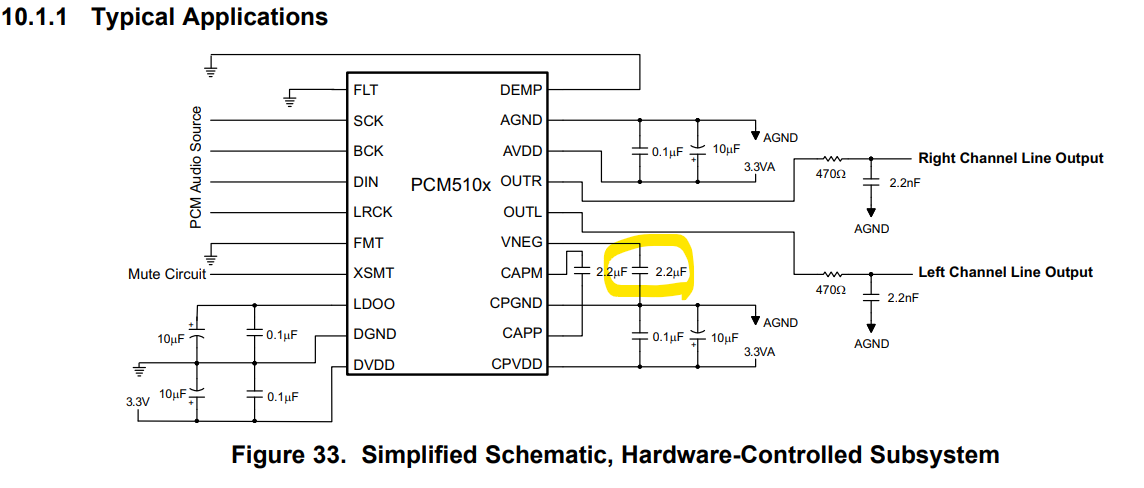
\includegraphics[width=0.8\textwidth]{obrazky/PCM5102A_typical_application.png}
    \caption{Typické zapojení PCM510x}
    \label{fig:PCM5102A_typical_application}
\end{figure}

Obsahuje integrovanou nábojovou pumpu - vytváří záporné napájecí napětí přestože je čip krmen 3,3 V. DAC má pak soustředěný výstup kolem 0V.
Ale je zapotřebí přidat kondenzátor mezi CAPP a CAPM piny (2 a 4, používá se pro přenos náboje), a potom ještě jeden mezi VNEG a CPGND piny (5 a 3, filtruje vztvořené záporné napětí).

PIN 10 DEMP na GND, vypne se tam de-emphasis.

PIN 11 FLT na GND, takže je použít normální FIR filtr.

PIN 12 SCK na GND, takže je použít interní PLL bez externího MCLK

PIN 16 FMT na GND, jde o standardní I2S formát.

PIN 17 XSMT, připojen na 3,3V.


- Čip využívá Direct Path, nepotřebuje na audio výstupu oddělovací kondenzátory, protože výstup už kmitá kolem nuly (GND). Ale aby toho byl schopen dosáhnout pomocí napětí +3,3 V, musí si vytvořit i záporné napětí -3,3 V (VNEG větev). C22 mezi piny CAPP a CAPM (flying capacitor), má dvě fáze. V první fázi se nabije na 3,3 V, ve druhé fázi se přepne mezi GND a pin VNEG (přelije náboj do záporné větve). - Hodnota převzaná od Texas Instruments.

- C23 mezi VNEG a CPGND je vyhlazovací kondenzátor záporného napětí, udržuje stabilních -3,3 V vůči zemi. 

- C24 - analogový výstupní filtr RC

- C25 - analogový výstupní filtr RC

- C26 - nízká parazitní indukčnost, odvádí ryché proudové špičky - doporučeno TI

- C27 - dobrý na pomalejší změny odběru proudu - doporučeno TI

- C28 (100 nF, potlačuje rychlé rušení vznikající při spínání nábojové pumpy) a C29 (10 uF, stabilizuje 3,3 V napájení) - protože pin CPVDD odebírá proud v pulzech, pulzy mohou vytvoři rušení - hodnoty převzaté z doporučení Texas Instruments.

- C30 a C 31 - stejně jako u C26 a C27.

- C32 - filtrace a stabilizace interního LDO (interního napěťového regulátoru, vytářející cca 1,8 V z 3,3 V pro )

- C33 - filtrace vf 

\subsubsection{Výstupní analogový filtr RC}

- kondenzátory C24, C25 filtrují vf složky pro každý kanál do země -> filtr dolní propust
- aby filtr neovlivnil amplitudu/fázi slyšitelných vyšších tónů, volí se mezní frekvence 7 krát až 10 krát vyšší než 20 kHz. Hlavně je zapotřebí vyfiltrovat frekvence v MHz
- hodnoty rezistory C22 a C23 jsou natolik nízké, že neovlivní úbytek sigálu na vstupní impedanci běžného koncového zesilovače.

$ f_c = \frac{1}{2\pi R C} = \frac{1}{2\pi \cdot 470 \cdot 2{,}2 \cdot 10^{-9}} \approx 154 kHz$

\subsubsection{Sluchátkový zesilovač TPA6111A2D}
Zesílení analogového stereofonního signálu z D/A převodníku PCM5102A je docíleno pomocí integrovaného sluchátkového zesilovače TPA6111A2D od Texas Instruments. Obvod obsahuje dva nezávislé zesilovací kanály v invertujícím zapojení, umožňuje provoz při 3,3 V. 

Zesílení jednotlivých kanálů je určeno poměrem zpětnovazebního rezistoru $R_F$ a vstupního rezistoru $R_I$, platí vztah 
$A_v=-\frac{R_F}{R_I}$, kde pro $R_F$ i $R_I$ jsou zvoleny hodnoty 20 kohm, tedy $A_v=-\frac{20 komh}{20 kohm}=-1$. Napěťové zesílení se tedy rovná jedné, rovno zesílení 0 dB, nedochází k změně amplitudy. Záporné znaménko zde vyjadřuje fázovou inverzi o 180 stupňů. Zvolená konfigurace odpovídá doporučenému zapojení uvedené v technické dokumentaci dané součástky.

Ekvivalentní odpor působící na invertující vstup zesilovače je dán paralelní kombinací $R_F$ a $R_I$, $R_{\mathrm{eq}}=\frac{R_F R_I}{R_F+R_I}
=10,\mathrm{k}\Omega$, tato hodnota je v rámci doporučení výrobcem, tedy od 5 kOhm do 20 kOhm.

Při návrhu bylo zohledněno rozdílné napěťové rozmezí výstupních signálů D/A převodníku a sluchátkového zesilovače. Převodník PCM5102A při plném vybuzení dosahuje výstupní úrovně 2,1 V RMS (5,94 V špička špička, mnohem více, než zesilovač dokáže reprodukovat bez zkreslení). Regulace hlasitosti bude proto řícena digitálním útlumem PCM vzorků v mikrokontroléru STM32. Maximální úroveň bude stanovena s ohledem na výstupní napěťový rozkmit zesilovače, s ohledem na impedanci připojených sluchátek\dots

Ostatní komponenty ve schématu okolo TPA6111A2D

Vstupní vazební kondenzátory C38 a C39 (1 µF), sériově zapojeny mezi výstupy D/A převodníku a vstupy zesilovače, oddělující stejnosměrné složky signálu. Společně se vstupními rezistory R24 a R26 vytváření RC filtr horní propusti, určující dolní mezní kmitočet přenosové charakteristiky = 8 Hz.

\begin{equation}
    f_c = \frac{1}{2\pi R_I C_I}
    = \frac{1}{2\pi \cdot 20 \times 10^3 \cdot 1 \times 10^{-6}}
    \approx 7{,}96\,\mathrm{Hz}
    \label{eq:mezni_frekvence_vstup}
\end{equation}

Kondenzátor C34 o kapacitě 1 uF, ovlivňuje časový průběh náběhu interního předpětí, čímž omezuje vznik nechtěných impulzů při zapnutí zesilovače.

Blokovací kondenzátory C37 (potlačující vysokofrekvenční rušení a rychlé napěťové přechody), C40, zlepšují stabilitu napájení a omezují nežádoucí vlivy napájecího rušení na výstupní audio signál.
\begin{equation}
    X_C = \frac{1}{2\pi f C}
    \label{eq:kapacitni_reaktance}
\end{equation}
S rostoucí frekvencí klesá kapacitní reaktance, kondenzátor představuje pro vf složky nízkoimpedanční cestu ke GND. 

Výstupní vazební kondenzátory C17, C18 polarizované elektrolytické, zabraňují průchodu stejnosměrné složky do připojených sluchátek. Zvolená kapacita 470 µF pro sluchátka o impedanci 32 Ohm odpovídá dolní mezní frekvenci 10,58 Hz, podle 
\begin{equation}
    f_c = \frac{1}{2\pi R_L C_{\mathrm{out}}}
    = \frac{1}{2\pi \cdot 32 \cdot 470 \times 10^{-6}}
    \approx 10{,}58\,\mathrm{Hz}
    \label{eq:mezni_frekvence_vystup}
\end{equation}


\section{Paměťová část}
\label{section_pametova_cast}
V sekci úložiště je využit DM3AMT-ST-PEJM5 konektor typu push-push; vložení i vysunutí Micro SD karty se provádí stisknutím karty, konektor brázní samovolnému vypadnutí. Výrobce Hirose uvádní i ochranu proti obrácenému zasunutí karty \cite{datasheet_hirose_dm3}. 

Piny \texttt{DET\_B}  a \texttt{DET\_A} nejsou elektricky spojeny s kartou, pouze tvoří vývody mechanického spínače. Spínač sepne jestliže je karta plně zasunuta a mikrokontrolér ze signálu \texttt{SD\_DET} určí přítomost karty a zahájí její čtení nebo případně další manipulaci s daty. Bez karty je spínač rozepnutý, přes pull-up rezistor R21 neteče žádný proud a nevzniká zde ani úbytek napětí. GPIO mikrokotroléru čte ze signálu \texttt{SD\_DET} logickou 1. Jakmile je karta zasunuta, spínač uzel spojí se zemí a logická 0, napětí na uzlu je nulové (GND), a přes R21 teče proud a cca 70 \textmu A podle \ref{sd_karta_vypocet_proudu}. 
\begin{equation}
    I_{\mathrm{DET}} = \frac{U_{\mathrm{CC}}}{R_{21}}
    = \frac{3{,}3\,\mathrm{V}}{47\,\mathrm{k}\Omega}
    \approx 70\,\mathrm{\mu A},
    \label{sd_karta_vypocet_proudu}
\end{equation}
Pull-up rezistor je zde nutný, protože spínač umí uzel pouze stáhnout k zemi, nikoliv jej vytáhnout nahoru. Detekce karty je také možná přes pin 1 \texttt{DAT3}, ale jeho funce může být uživatelem nastavena jinak než je jeho zamýšlená funkce; navíc koliduje s 4bitovým režimem. Mechanický spínač zde bude mít zákmity, signál \texttt{SD\_DET} by bylo potřeba filtrovat přes RC článek, avšak pro tuto práci byla zvolena softwarová filtrace, cca 10-50 ms debounce, bude doplněno v následující bakalářské práci. Jak bylo zmíněno, podle \ref{sd_karta_vypocet_proudu} teče zde neustálý proud, u bateriového zařízení je tato spotřeba nezanedbatelná. Sekce o spotřebě bude více rozebíraná v následující práci.

Pull-up rezistory se podle \cite{manual_sandisk_microsd} musí umisťovat externě uživatelem, a to na všechny signály kromě hodinového signálu \texttt{SD\_CLK}. Je zde i možnost pro nterní pull-up rezistory v STM32, ale ty mohou být příliš slabé nebo mohou být krátkodobě odpojovány při změně konfigurace rozhraní, vedoucí k chybám komunikace mezi mikrokontrolérem a samotnou SD kartou. Hodnota pull-up rezistoru musí být podle \cite[s.~4]{an2111_swissbit} v  rozsahu od 10\,k$\Omega$ do 100\,k$\Omega$. V navrženém zapojení jsou osazeny rezistory R16 až R20 s hodnotou 47\,k$\Omega$, tedy hodnoty rezistoru splňují doporučení pro datové vodiče \cite[s.~4]{an2111_swissbit}, \cite[s.~3-8, tab.~3-5]{manual_sandisk_sd}. Vyšší hodnota snižuje klidový odběr zatímco rychlost sběrnice neomezuje, hrany signálů aktivně tvoří budiče typu push-pull \cite[s.~15]{manual_sandisk_microsd}. Stejnou hodnotu používá i referenční návrh vývojové desky výrobce mikrokontroléru \cite[s.~44, obr.~28]{um2411_st}.

Kondenzátor C20 s hodnotou 100\,nF je umístěn co nejblíže k vývodu VDD SD karty. Pokrývá rychlé proudové odběry, jelikož bulk kondenzátor C13 nemusí dostatečně rychle dodat náboj; indukčnost napájecího spoje mezi ním a vývodem karty zpomaluje rychlost změny proudu. C13 s hodnotou 22\,\textmu F slouží jako zásobník, výše zmíněný bulk.


SD karta má vlastní řadič a paměť typu NAND flash. Zápis a mazání v paměti NAND vyžadují napětí vyšší, než je napájecí, které si karta vytváří vnitřními nábojovými pumpami \cite[kap.~11]{micheloni_nand}. Tyto pumpy se aktivují v dávkách, řadič navíc paralelně pracuje s více bloky, odběr tak není plynulý, ale je impulzní s charakterem opakujících se špiček. Jestliže během špiček napětí na vývodu VDD klesne pod práh detekce podpětí (tedy klesne na napětí, které řadič vyhodnotí jako nedostatečné pro napájení), je řadičem vyhodnocen stav výpadku napájení a zablokuje zápis na kartu. Jde o ochranu dat, přerušení programovacího cyklu NAND by poškodilo zapisovaná data. Při inicializaci karty je princip podobný. Inicializace se rozběhne, při proudové špičce napětí poklesne, karta se resetuje a celý cyklus se opakuje. Pokles napětí na kondenzátoru při skoku odebíraného proudu je 
\begin{equation}
    \Delta U = \frac{I\,\Delta t}{C},
    \label{sd_karta_pokles_napeti}
\end{equation} kde $I$ je odebíraný proud, $\Delta t$ doba jeho trvání
a $C$ kapacita kondenzátoru. Celou špičku však kondenzátor pokrýt nemůže: pro
$I = 300$\,mA a $\Delta t = 1$\,ms by podle vztahu~\eqref{sd_karta_pokles_napeti} vyšel pokles 13,6\,V. Po většinu trvání špičky proto proud dodává měnič TPS63070 a kondenzátor C13 omezuje pokles napětí pouze do okamžiku, než zareaguje zpětnovazební regulační smyčka měniče. Pro dobu odezvy $\Delta t = 10$\,\textmu s vychází
\begin{equation}
    \Delta U = \frac{0{,}3\,\mathrm{A} \cdot
    10\,\mathrm{\mu s}}{22\,\mathrm{\mu F}}
    \approx 0{,}14\,\mathrm{V},
    \label{sd_karta_pokles_vypocet}
\end{equation}
což je vzhledem k povolenému rozsahu napájecího napětí karty 2,7 až 3,6\,V přijatelné.

Slot microSD karty je uživatelsky přístupný konektor, jde tedy o typické vstupní místo elektrostatického výboje (ESD). ST uvádí, že právě nejčastějšími vstupními body pro ESD jsou konektory, proto jsou osazeny U7 a U8, oba USBLC6-4SC6, oba chránící čtyři vodiče (součástka je dostupná pouze ve čtyřkanálovém provedení, jeden kanál zůstává proto nezapojený). Dále uvádí, že ochrana má být co nejblíže k očekávanému místu výboje a má ležet přímo na signálové a zemní cestě, aby proud protekl ochranou a ne mikrokontrolérem \cite{an5612_st}. Dvojice součástek v pouzdře SOT23-6L navíc umožňuje umístit ochranu blíže k chráněným vodičům, než by dovolilo jediné pouzdro s osmi kanály. Součáskta byla zvolena kvůli své vlastní nízké kapacitě 3\,pF typicky a 4\,pF maximálně \cite{datasheet_usblc6}. Samotná karta smí mít nejvýše 10\,pF a celková kapacita vodiče sběrnice je omezena na 250\,pF, respektive 100\,pF \cite[s.~3-8, tab.~3-5]{manual_sandisk_sd}. Každý vodič je připojen dvojicí diod k napájecí a zemnící větvi. Vývod \texttt{VBUS} je proto připojen na napájecí napětí 3,3\,V a kondenzátor C41 zajišťuje nízkou impedanci této větve pro svedený výbojový proud \cite{datasheet_usblc6}.


\section{Část uživatelského rozhraní}
Tlačítka pro spuštění a zastavení přehrávání, přesun na další a předchozí skladbu a tlačítka pro ovládání hlasitosti nejsou zapojena s externími pull-up rezistory, klidovou úroveň zajišťují vnitřní pull-up rezistory mikrokontroléru. Na rozdíl od sběrnice paměťové karty zde krátkodobé odpojení vnitřního pull-up rezistoru v mikrokontroléru při změně konfigurace nemůže narušit komunikaci, vodič spojuje pouze jeden vstup mikrokontroléru a jeden spínač. Zákmity kontaktů budou řešeny softwarově v navazující práci, stejně jako v kapitole~\ref{section_pametova_cast}.

Signál \texttt{OLED\_CS} je rezistorem R32 o hodnotě 10\,k$\Omega$ připojen k napájecímu napětí 3,3\,V. Po resetu mikrokontroléru nejsou vývody GPIO nakonfigurovány jako výstupy a nacházejí se ve stavu vysoké impedance, signál \texttt{OLED\_CS} by plaval. Řadič displeje by mohl náhodnou úroveň na sběrnici vyhodnotit jako platný přenos. Rezistor R32 udržuje tento signál v neaktivní vysoké úrovni, dokud jej firmware nepřevezme. Napájení displeje blokují kondenzátory C62 o hodnotě 100\,nF a C63 o hodnotě 4,7\,\textmu F. Kondenzátor C62 je umístěn co nejblíže k napájecímu vývodu modulu a pokrývá rychlé změny odebíraného proudu, C63 slouží jako místní zásobník náboje

Výrobce displeje nezveřejňuje rozměrovou dokumentaci, rozteč vývodů, poloha montážních otvorů a obrysové rozměry byly proto odměřeny na zakoupeném vzorku a podle nich bylo vytvořeno vlastní pouzdro \texttt{OLED\_SPI\_7pin\_P2.54mm}.
